
\subsection{Punto \textbf{1}}

\begin{itemize}
\item \emph{\textbf{Estimar con cálculo manual el retardo del inversor \textbf{CMOS} cuando está cargado por otro inversor idéntico. Considerar los efectos de canal corto.}}
\end{itemize}


Para la obtención del tiempo de retardo, se asume un modelo RC, de donde el tiempo buscado se determinará como el tiempo de carga del capacitor equivalente a través del resistor equivalente.



En el cuadro~\tableref{table:device_parameters}, se pueden ver resumidos los parámetros de los dispositivos para el proceso \textbf{SAED-90}.



\begin{table}[H]  %%\centering

    \setlength\arrayrulewidth{1.5pt}
    \arrayrulecolor{white}
    \def\clinecolor{\hhline{|>{\arrayrulecolor{white}}-%
    >{\arrayrulecolor{white}}|-|-|-|-|-|-|-|-|-|-|}}
\resizebox{0.80 \textwidth}{!}{% 
       
\begin{tabularx}{1 \textwidth}%
    {|
    >{\columncolor{white} \centering\arraybackslash}m{0.06\textwidth}
     |
    >{\columncolor{white} \centering\arraybackslash}m{0.104\textwidth}
     |
    >{\columncolor{white} \centering\arraybackslash}m{0.104\textwidth}
     |
    >{\columncolor{white} \centering\arraybackslash}m{0.104\textwidth}
     |
    >{\columncolor{white} \centering\arraybackslash}m{0.104\textwidth}
     |
    >{\columncolor{white} \centering\arraybackslash}m{0.104\textwidth} 
     |
    >{\columncolor{white} \centering\arraybackslash}m{0.104\textwidth}  
     |
    >{\columncolor{white} \centering\arraybackslash}m{0.104\textwidth}  
     |
    >{\columncolor{white} \centering\arraybackslash}m{0.104\textwidth} 
     |
    >{\columncolor{white} \centering\arraybackslash}m{0.104\textwidth} 
     |     
    }
    \rowcolor{HeadersColor} \cellcolor{white} \thead{}  & \thead{$t_{ox}$} & \thead{$V_{th}$} & \thead{$I_{D_{sat}}$} & \thead{$\mu \cdot C_{ox}$} & \thead{$X_{j}$} & \thead{$\gamma$} & \thead{$C_{ov}$} & \thead{$C_{j}$} & \thead{$C_{j_{sw}}$} \\  
    \hhline{|-|-|-|-|-|-|-|-|-|-|}
    \rowcolor{gray!20} \cellcolor{gray!40} \textbf{NMOS} & $2.05 \si[per-mode=symbol]{\micro\meter}$ & $397 \si[per-mode=symbol]{\milli\volt}$ & $869 \si[per-mode=symbol]{\micro\ampere\per\micro\meter}$ & $428 \si[per-mode=symbol]{\micro\ampere\per\volt\squared}$ & $415 \si[per-mode=symbol]{\micro\meter}$ & $0.4 \si[per-mode=symbol]{\volt\tothe{0.5}}$ & $0.26 \si[per-mode=symbol]{\femto\farad\per\micro\meter}$ &  $0.5 \si[per-mode=symbol]{\femto\farad\per\micro\meter\squared}$ & $0.5 \si[per-mode=symbol]{\femto\farad\per\micro\meter}$ \\
    \hhline{|-|-|-|-|-|-|-|-|-|-|}
    \rowcolor{gray!20} \cellcolor{gray!40} \textbf{PMOS} & $2.15 \si[per-mode=symbol]{\micro\meter}$ & $-276 \si[per-mode=symbol]{\milli\volt}$ & $-426 \si[per-mode=symbol]{\micro\ampere\per\micro\meter}$ & $-124 \si[per-mode=symbol]{\micro\ampere\per\volt\squared}$ & $28 \si[per-mode=symbol]{\micro\meter}$ & $0.4 \si[per-mode=symbol]{\volt\tothe{0.5}}$ & $0.26 \si[per-mode=symbol]{\femto\farad\per\micro\meter}$ &  $0.5 \si[per-mode=symbol]{\femto\farad\per\micro\meter\squared}$ & $0.5 \si[per-mode=symbol]{\femto\farad\per\micro\meter}$ \\
    \end{tabularx}}
	\caption{\footnotesize{Parámetros de los dispositivos.}}
	\label{table:device_parameters}
\end{table}





En la figura~\figref{fig:fig_inverter_loaded_with_inverter} puede verse el circuito a implementar, y en la figura~\figref{fig:fig_inverter_loaded_with_inverter_capacitances} pueden versse todas las capacidades a tener en cuenta en los cálculos a realizar.


\begin{figure}[H] %htb
\begin{center}
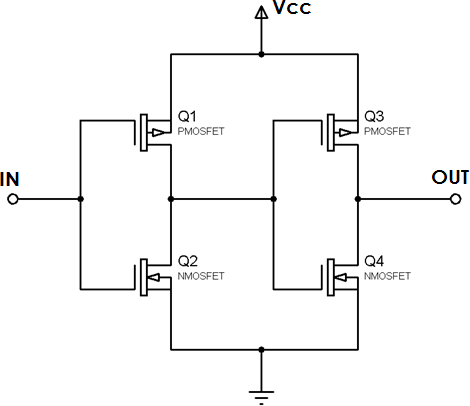
\includegraphics[width=0.3 \textwidth, angle=0]{./img/point1/inverter_loaded_with_inverter}
\caption{\label{fig:fig_inverter_loaded_with_inverter}\footnotesize{Inversor \textbf{CMOS} cargado con un inversor idéntico.}}
\end{center}
\end{figure}



\begin{figure}[H] %htb
\begin{center}
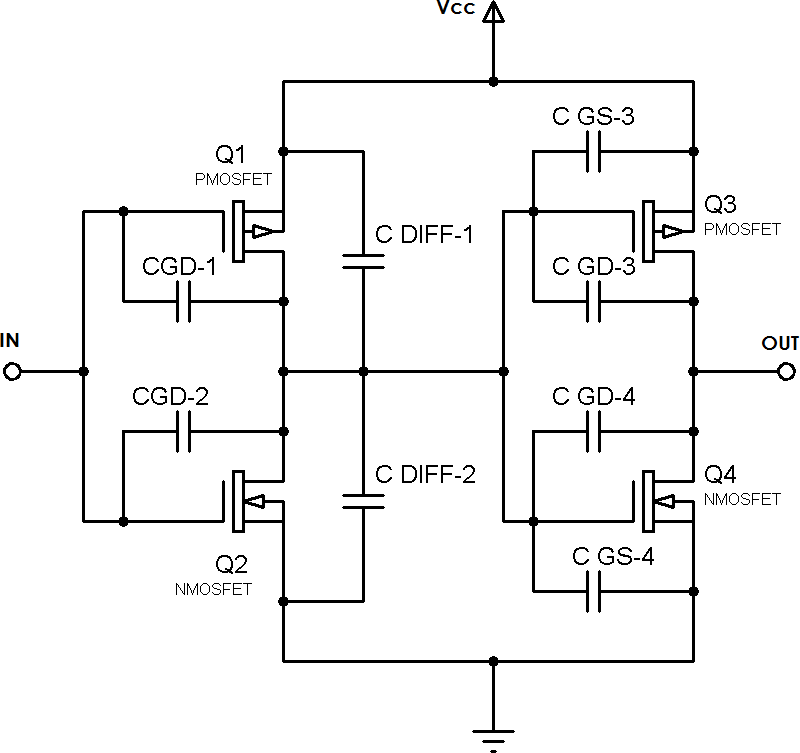
\includegraphics[width=0.3 \textwidth, angle=0]{./img/point1/inverter_loaded_with_inverter_capacitances}
\caption{\label{fig:fig_inverter_loaded_with_inverter_capacitances}\footnotesize{Inversor \textbf{CMOS} cargado con un inversor idéntico (capacidades tenidas en cuenta).}}
\end{center}
\end{figure}



\vfill

\clearpage


\subsubsection{Determinación la capacidad de carga equivalente $C_{L}$}


De la figura~\figref{fig:fig_inverter_loaded_with_inverter_capacitances}, se obtiene que la capacidad que carga al primer inversor es:



\begin{equation}
C_{L} = \left( 2 \cdot C_{GD_{2}} + C_{diff_{2}} \right) + \left( 2 \cdot C_{GD_{1}} + C_{diff_{1}} \right) + \left( 2 \cdot C_{GD_{4}} + C_{GS_{4}} + C_{G_{4}} \right) + \left( 2 \cdot C_{GD_{3}} + C_{GS_{3}} + C_{G_{3}} \right)
\end{equation}


Donde se identifican:


\begin{equation*}
C_{out_{inv_{1}}} = \left( 2 \cdot C_{GD_{2}} + C_{diff_{2}} \right) + \left( 2 \cdot C_{GD_{1}} + C_{diff_{1}} \right)
\end{equation*}


\begin{equation*}
C_{L_{inv_{2}}} = \left( 2 \cdot C_{GD_{4}} + C_{GS_{4}} + C_{G_{4}} \right) + \left( 2 \cdot C_{GD_{3}} + C_{GS_{3}} + C_{G_{3}} \right)
\end{equation*}


Siendo entonces:


\begin{equation*}
C_{L} = C_{out_{inv_{1}}} + C_{L_{inv_{2}}}
\end{equation*}



\subsubsection{Cálculo de la capacidad de salida del inversor 1, $C_{out_{inv_{1}}}$}


\begin{equation*}
C_{out_{inv_{1}}} = \left( 2 \cdot C_{GD_{2}} + C_{diff_{2}} \right) + \left( 2 \cdot C_{GD_{1}} + C_{diff_{1}} \right)
\end{equation*}


Las capacidades $C_{GD_{1}}$ y $C_{GD_{2}}$, son las capacidades de overlap, reflejadas a la entrada.


\begin{equation*}
C_{GD_{i}} = 2 \cdot W_{i} \cdot C_{ov_{i}}  \; \; \;   i \in \{ 1, 2 \}
\end{equation*}


Tengo además:

\begin{equation*}
W_{2}= W_{N} = 0.92 \si[per-mode=symbol]{\micro\meter}
\end{equation*}

\begin{equation*}
W_{1}= W_{P} = 2 \cdot W_{N} = 1.84 \si[per-mode=symbol]{\micro\meter}
\end{equation*}

Y usando los datos del cuadro~\tableref{table:device_parameters}, $C_{ov_{N}}$ y $C_{ov_{P}}$

Obtengo:


\begin{equation*}
\boxed{ C_{GD_{1}} = 0.4784 \si[per-mode=symbol]{\femto\farad} }
\end{equation*}


\begin{equation*}
\boxed{ C_{GD_{2}} = 0.2392 \si[per-mode=symbol]{\femto\farad} }
\end{equation*}


Las capacidades $C_{diff_{1}}$ y $C_{diff_{2}}$, son las capacidades de juntura, que se calculan refiriéndose a lo que se puede apreciar en la figura~\figref{fig:fig_mosfet_structure}.



\begin{figure}[H] %htb
\begin{center}
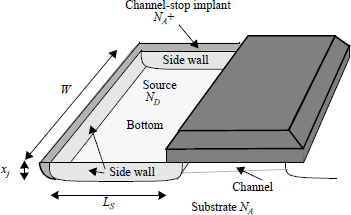
\includegraphics[width=0.7 \textwidth, angle=0]{./img/point1/mosfet_structure}
\caption{\label{fig:fig_mosfet_structure}\footnotesize{Estructura del MOSFET.}}
\end{center}
\end{figure}



Tengo entonces en forma genérica para ambos dispositivos, \textbf{NMOS} y \textbf{PMOS}:

\begin{equation*}
C_{diff} = C_{bottom} + C_{side\_wall}
\end{equation*}

Luego:

\begin{equation*}
C_{diff} = C_{j} \cdot Area + C_{j_{sw}} \cdot perim
\end{equation*}


Y usando los datos del cuadro~\tableref{table:device_parameters}, $C_{j_{N}}$, $C_{j_{sw_{N}}}$ y $C_{j_{P}}$, $C_{j_{sw_{P}}}$. Y con:

\begin{equation*}
L_{s_{N}} = L_{s_{P}} = 0.3 \si[per-mode=symbol]{\micro\meter}
\end{equation*}

\begin{equation*}
W_{1}= W_{P} = 2 \cdot W_{N} = 1.84 \si[per-mode=symbol]{\micro\meter}
\end{equation*}


\begin{equation*}
W_{2}= W_{N} = 0.92 \si[per-mode=symbol]{\micro\meter}
\end{equation*}


Obtengo:

\begin{equation*}
\boxed{ C_{diff_{1}} = 0.276 \si[per-mode=symbol]{\femto\farad} + 1.22 \si[per-mode=symbol]{\femto\farad} = 1.496 \si[per-mode=symbol]{\femto\farad} }
\end{equation*}


\begin{equation*}
\boxed{ C_{diff_{2}} = 0.138 \si[per-mode=symbol]{\femto\farad} + 0.76 \si[per-mode=symbol]{\femto\farad} = 0.898 \si[per-mode=symbol]{\femto\farad} }
\end{equation*}



Finalmente:

\begin{equation*}
\boxed{ C_{out_{inv_{1}}} = \left( 2 \cdot 0.2392 \si[per-mode=symbol]{\femto\farad} + 0.898 \si[per-mode=symbol]{\femto\farad} \right) + \left( 2 \cdot 0.4784 \si[per-mode=symbol]{\femto\farad} + 1.496 \si[per-mode=symbol]{\femto\farad} \right) = 3.8292 \si[per-mode=symbol]{\femto\farad} }
\end{equation*}



\subsubsection{Cálculo de la capacidad de carga que agrega el inversor 2, $C_{L_{inv_{2}}}$}


\begin{equation*}
C_{L_{inv_{2}}} = \left( 2 \cdot C_{GD_{4}} + C_{GS_{4}} + C_{G_{4}} \right) + \left( 2 \cdot C_{GD_{3}} + C_{GS_{3}} + C_{G_{3}} \right)
\end{equation*}


Para las capacidades $C_{GD_{i}}$, que son las capacidades de overlap, tengo:

\begin{equation*}
\boxed{ C_{GD_{3}} = C_{GD_{1}} = 0.47 \si[per-mode=symbol]{\femto\farad} }
\end{equation*}


\begin{equation*}
\boxed{ C_{GD_{4}} = C_{GD_{2}} = 0.24 \si[per-mode=symbol]{\femto\farad} }
\end{equation*}



Para las capacidades $C_{G_{i}}$, tengo:

\begin{equation*}
\boxed{ C_{G_{3}} = C_{G_{P}} = C_{ox} \cdot W_{P} \cdot L_{s_{P}} = 3.2 \si[per-mode=symbol]{\femto\farad\per\micro\meter\squared} \cdot 1.84 \si[per-mode=symbol]{\micro\meter} \cdot 1.3 \si[per-mode=symbol]{\micro\meter} = 7.6544 \si[per-mode=symbol]{\femto\farad} }
\end{equation*}


\begin{equation*}
\boxed{ C_{G_{4}} = C_{G_{N}} = C_{ox} \cdot W_{N} \cdot L_{s_{N}} = 3.2 \si[per-mode=symbol]{\femto\farad\per\micro\meter\squared} \cdot 0.92 \si[per-mode=symbol]{\micro\meter} \cdot 1.3 \si[per-mode=symbol]{\micro\meter} = 3.8272 \si[per-mode=symbol]{\femto\farad} }
\end{equation*}



Donde la capacidad del óxido se calcula a partir del producto $\mu \cdot C_{ox}$, que es dato, y la movilidad correspondiente.



Para las capacidades $C_{GS_{i}}$ tengo:


\begin{equation*}
\boxed{ C_{GS_{3}} = C_{GS_{P}} = W_{P} \cdot C_{ov_{P}} = 1.84 \si[per-mode=symbol]{\micro\meter} \cdot 0.26 \si[per-mode=symbol]{\femto\farad\per\micro\meter} = 0.4784 \si[per-mode=symbol]{\femto\farad} }
\end{equation*}


\begin{equation*}
\boxed{ C_{GS_{4}} = C_{GS_{N}} = W_{P} \cdot C_{ov_{N}} = 0.92 \si[per-mode=symbol]{\micro\meter} \cdot 0.26 \si[per-mode=symbol]{\femto\farad\per\micro\meter} = 0.2392 \si[per-mode=symbol]{\femto\farad} }
\end{equation*}





Se obtiene finalmente:


\begin{equation*}
\boxed{ C_{L_{inv_{2}}} =  \left( 2 \cdot 0.24 \si[per-mode=symbol]{\femto\farad} + 0.2392 \si[per-mode=symbol]{\femto\farad} + 3.8272 \si[per-mode=symbol]{\femto\farad} \right) + \left( 2 \cdot 0.47 \si[per-mode=symbol]{\femto\farad} + 0.4784 \si[per-mode=symbol]{\femto\farad} + 7.6544 \si[per-mode=symbol]{\femto\farad} \right) = 13.6192 \si[per-mode=symbol]{\femto\farad} }
\end{equation*}



Con lo que podemos calcular ahora $C_{L}$:


\begin{equation*}
C_{L} = C_{out_{inv_{1}}} + C_{L_{inv_{2}}}
\end{equation*}


\begin{equation*}
\boxed{  C_{L} = 3.8292 \si[per-mode=symbol]{\femto\farad} + 13.6192 \si[per-mode=symbol]{\femto\farad} = 17.4484 \si[per-mode=symbol]{\femto\farad} }
\end{equation*}





\subsubsection{Determinación la resistencia de carga equivalente $R_{L}$}


Las resistencias equivalentes para cada estado del inversor, se muestran en la figura~\figref{fig:fig_inverter_equivalent_resistances}.




\begin{figure}[H] %htb
\begin{center}
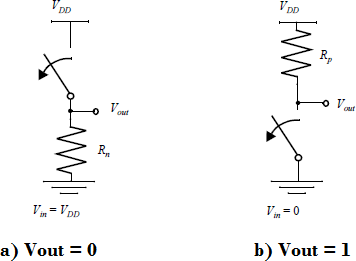
\includegraphics[width=0.7 \textwidth, angle=0]{./img/point1/resistance_equivalent}
\caption{\label{fig:fig_inverter_equivalent_resistances}\footnotesize{Resistencias equivalentes en cada estado del inversor \textbf{CMOS}.}}
\end{center}
\end{figure}



En cada estado, el transistor que conduce, se encuentra en la zona óhmica de operación, el valor de estas resistencias es represetando por $R_{P}$ y $R_{N}$. \\



Para obtener el valor de esta resistencia equivalente, se utiliza la expresión:


\begin{equation}
R_{eq} = \frac{3}{4} \cdot \frac{V_{DD}}{I_{D_{sat}}} \cdot \left( 1 - \frac{7}{9} \cdot \lambda \cdot V_{DD} \right)
\label{eq:eq_r_eq}
\end{equation} \\



La modulación del canal se produce cuando el transistor trabaja en la zona de saturación y en el canal, en la difusión del drenaje, se produce el efecto de  estrangulamiento del canal, como se muestra en la figura~\figref{fig:fig_channel_strangulation}.



\begin{figure}[H] %htb
\begin{center}
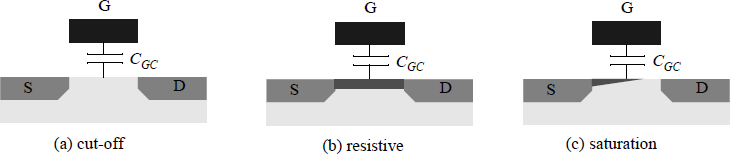
\includegraphics[width=0.7 \textwidth, angle=0]{./img/point1/channel_strangulation}
\caption{\label{fig:fig_channel_strangulation}\footnotesize{Estrangulación del canal.}}
\end{center}
\end{figure}


En la zona óhmica, no se tiene en cuenta el efecto de modulación del canal, esto es $\lambda = 0$, con lo que la expresión~\eqref{eq:eq_r_eq}, se reduce a:


\begin{equation}
R_{eq} = \frac{3}{4} \cdot \frac{V_{DD}}{I_{D_{sat}}}
\label{eq:eq_r_eq_red}
\end{equation} \\














